% Name: Rule of Sarrus
% Description: The determinant of a 3×3 matrix: copy the first two columns to the right, add the products down the three blue diagonals, and subtract those up the three orange ones.
% Tags: determinant, rule of Sarrus, 3×3 matrix, linear algebra

\usetikzlibrary{matrix}

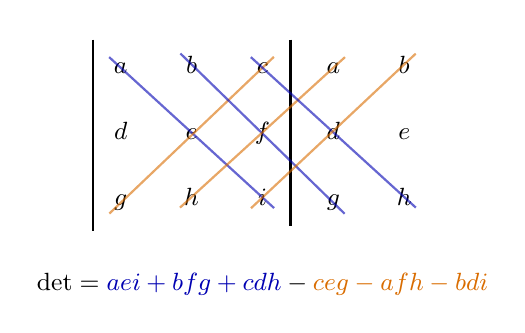
\begin{tikzpicture}[every node/.style={font=\small}]
  \matrix (m) [matrix of math nodes, nodes={minimum size=7mm}, column sep=2mm, row sep=1mm] {
    a & b & c & a & b \\
    d & e & f & d & e \\
    g & h & i & g & h \\
  };
  \draw[thick] (m-1-1.north west) -- (m-3-1.south west) (m-1-3.north east) -- (m-3-3.south east);
  \foreach \c [evaluate=\c as \d using int(\c+2)] in {1,2,3} {
    \draw[blue!70!black, thick, opacity=0.6, shorten <=-2mm, shorten >=-2mm] (m-1-\c.center) -- (m-3-\d.center);
    \draw[orange!85!black, thick, opacity=0.6, shorten <=-2mm, shorten >=-2mm] (m-3-\c.center) -- (m-1-\d.center);
  }
  \node[below=3mm, align=center] at (m.south) {$\det = {\color{blue!70!black} aei + bfg + cdh} - {\color{orange!85!black} ceg - afh - bdi}$};
\end{tikzpicture}
